\section{Оптимизация параллельного обхода ограничений для GPU} \label{ch3:chunks}
	В рамках данной работы, перед автором стояла задача не только разработке эвристического алгоритма описанного в главе \label{ch3:heuristic}, но и реализации, с использованием GPU. Действительно, главной отличительной особенностью GPU относительно CPU является много большее количество ядер процессора. Таким образом, учитывая закон Амдала, некоторые алгоритмы могут быть многократно ускорены за счет грамотного разбиения на подзадачи. Лучше всего GPU справляется в ситуации, когда вышеупомянутые задачи являются вычислительными задачами имеющими одинаковый алгоритм решения, однако разные входные данные. Подход, в котором GPU используется для вычисления не-графических задач принято называть GPGPU - General-purpose computing on graphics processing units. Для реализации данного подхода есть два пути: либо использование специализированной библиотеки для GPGPU (таких как Nvidia CUDA или OpenCL), либо использование вычислительных шейдеров в графических библиотеках (таких как DirectX12 или OpenGL). В рамках данной работы, автором рассматривается применение вычислительных шейдеров, так как конечной целью является встраивание симуляции тканей в приложение использующее DirectX12.
	
	Введем некоторые основные понятия программирования на GPGPU. Если говорить с точки зрения выполнения, то на GPU запускаются шейдеры. Шейдеры запускаются параллельно, имеют одинаковый код, но получают аргументом числанный номер своего потока. Потоки объединяются в группы, причем все группы имеет одинаковый размер. Программист же, при отправке команды на запуск какого-либо шейдера, указывает целое количество групп, которые он хочет вызвать. Для запуска каждой группы, GPU выделяет целое число $Wavefront$-ов - наборов из процессоров, которые выполняют операции абсолютно параллельно. В случае использования видеокарт Nvidia размер одного $Wavefront$-а равен 32, а в случае AMD 64.
	
	Если говорить с точки зрения памяти, каждый поток имеет локальную память (для локальных переменных шейдера), глобальную память (для считывания входных параметров и записи результирующих) и $groupshared$ память. Последняя является более быстрым по отношению к глобальной, однако выделяется только в рамках запуска одной группы и может быть использована потоками внутри группы для обмена данными.
	
	Если же говорить с точки зрения синхронизации, то в рамках языка HLSL и DirectX12, есть два вида синхронизации вычислительных шейдеров:
	\begin{enumerate}[1.]
		\item Применение барьера на глобальную память, в которую записывается результат. Таким образом следующие команды не начнут выполняться до тех пор, пока каждая группа не закончит записывать в данную память.
		\item Использование команды шейдера $GroupMemoryBarrierWithGroupSync$, которая позволяет синхронизировать все $Wavefront$-ы внутри одной группы.
	\end{enumerate}
	
	Рассмотрим алгоритм XPBD представленный на \firef{alg:HeuristicXPBD} и перепишем его в с точки зрения возможной параллелизации(\firef{alg:HeuristicParallelXPBD}).

\begin{algorithm} [h]
	\SetKwFunction{algoXPBDParallelPseudocode}{} 
	\SetKwProg{myalg}{Algorithm}{}{} %write in 2nd agrument <<Algorithm>>, <<Procedure>> etc
	\nonl\myalg{\algoXPBDParallelPseudocode}{
		\For{$\forall step \in 1..solverStep$}{			
			\If{$mod(step, HeuristicStep) = 0$}
			{
				\lForPar{$getHorRopes()$}
				{
					$HeuristicAlgorithm()$
				}
				
				$syncPoint()$
				
				\lForPar{$getVerRopes()$}
				{
					$HeuristicAlgorithm()$
				}
			}
			
			\lForPar{$getParticles()$}
			{
				$predictParticle()$
			}
			
			$syncPoint()$
			
			\lForPar{$getParticles()$}
			{
				$generateCollisionConstraint()$
			}
			
			$syncPoint()$
			
			\For{$\forall type \in \{structural, shear, bending\}$}
			{
				\For{$\forall color \in getColors(type)$}
				{
					\ForPar{$getConstraints(type, color)$}
					{
						$solveXPBDConstraint()$
					}
					
					$syncPoint()$
				}				
			}
			
			\ForPar{$getCollisionConstraints()$}
			{
				$solveCollisionConstaint()$
			}
			
			$syncPoint()$	
						
			\lForPar{$getParticles()$}
			{
				$saveNewParticlePos()$
			}		
			
			$syncPoint()$
		}
	}
	\caption{Псевдокод алгоритма Extended Position Based Dynamics с использованием Small steps, эвристического алгоритма и размеченными местами возможной параллелизации}\label{alg:HeuristicParallelXPBD}
\end{algorithm}

	Как можно заметить, данный алгоритм отлично разбивается на подзадачи имеющие одинаковый алгоритм но разные входные данные, что прекрасно ложится на использование технологии GPGPU. Однако возникает вопрос: как именно представить данный алгоритм при помощи GPU.
	
	Первый вариант: представить весь этот алгоритм как единый шейдер, для которого будет запущена только одна группа (данное решение используется в NVidia Cloth). Тогда каждый $syncPoint$ будет представлен как вызов $GroupMemoryBarrierWithGroupSync$, а частицы и ограничения сначала должны быть загружены в $groupshared$ память, а после данного алгоритма выгружены обратно в глобальную. Недостатком данного подхода является то, что размер группы в языке HLSL не может превышать 1024, а значит невозможно использовать более 1024 потоков.
	
	Второй вариант: представить каждый \say{\textbf{for} * \textbf{do in parallel}} как отдельный шейдер. Тогда каждый $syncPoint$ будет представлен как выставление барьера. Недостатком данного подхода является то, что не используется $groupshared$ память, тем алгоритм теряет в производительность на постоянной записи и чтении из глобальной памяти. Также, недостатком является частая смена и вызов различных шейдеров, что привносит дополнительные расходы по времени выполнения.
	
	В рамках исследования алгоритма XPBD с использованием техники Small steps и обходом ограничений используя реберную раскраску было замечено, что в течении одной итерации вляние частиц ограничено. Это означает, что для подсчета положения конкретной частицы на следующей итерации необходимо знать положение лишь некоторых соседних частиц, а не всей ткани.
	
	Для определения границ влияния частиц, был поставлен следующий эксперимент
	\begin{enumerate}[1.]
		\item Строится сетка размером $(N+2)$ на $(N+2)$ вершины, соединенные между собой аналогично тому, как частицы ткани соединены структурными ограничениями
		\item Внешние вершины сетки отмечаются красным цветом, в то время как внутренние ограничения помечаются синим
		\item В том же порядке, в котором обрабатываются структурные ограничения в ткани, обрабатываем ребра в сетке по следующему алгоритму: если одна из вершин красная, то перекрашиваем вторую вершину в красный цвет
	\end{enumerate}
	
	Пример данного эксперимента можно увидеть на \firef{fig:chunkStructExp}
	
	\begin{figure}[ht]
		\adjustbox{minipage=1.3em,valign=t}{\subcaption{}\label{fig:chunkStruct-color0}}%
		\begin{subfigure}[t]{\dimexpr.5\linewidth-1.3em\relax}
			\centering
			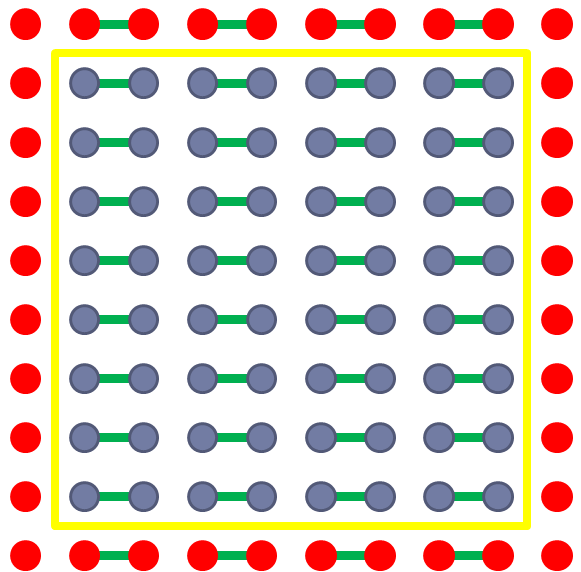
\includegraphics[width=.65\linewidth,valign=t]{my_folder/images/chunk_structural_1}
		\end{subfigure}
		\hfill %выровнять по ширине
		\adjustbox{minipage=1.3em,valign=t}{\subcaption{}\label{fig:chunkStruct-color1}}%
		\begin{subfigure}[t]{\dimexpr.5\linewidth-1.3em\relax}
			\centering
			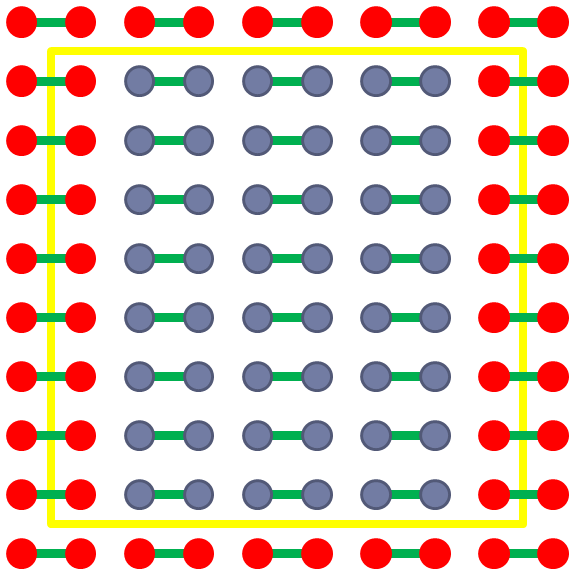
\includegraphics[width=.65\linewidth,valign=t]{my_folder/images/chunk_structural_2}
		\end{subfigure}
		\\[20pt]	
		\adjustbox{minipage=1.3em,valign=t}{\subcaption{}\label{fig:chunkStruct-color2}}%
		\begin{subfigure}[t]{\dimexpr.5\linewidth-1.3em\relax}
			\centering
			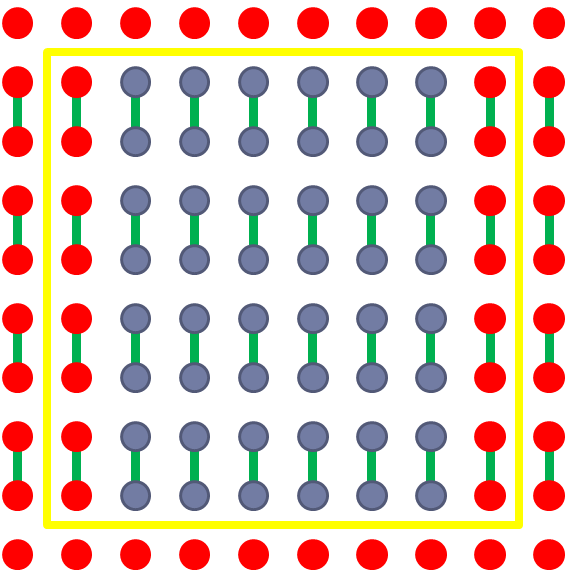
\includegraphics[width=.65\linewidth,valign=t]{my_folder/images/chunk_structural_3}
		\end{subfigure}%
		\hfill %выровнять по ширине
		\adjustbox{minipage=1.3em,valign=t}{\subcaption{}\label{fig:chunkStruct-color3}}%
		\begin{subfigure}[t]{\dimexpr.5\linewidth-1.3em\relax}
			\centering
			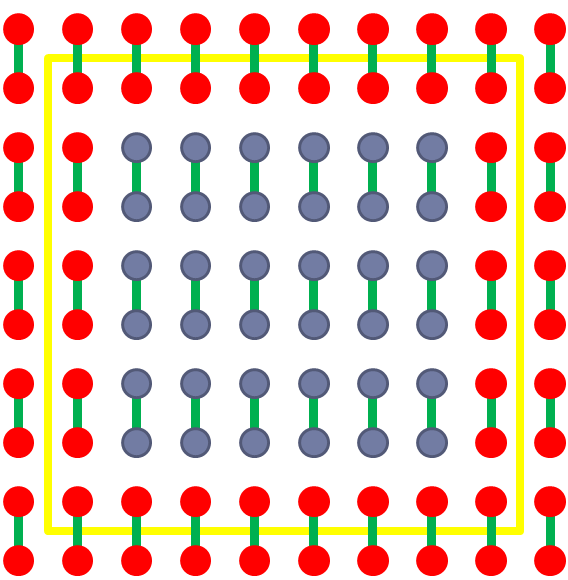
\includegraphics[width=.65\linewidth,valign=t]{my_folder/images/chunk_structural_4}
		\end{subfigure}
		\captionsetup{justification=centering} %центрировать
		\caption{Визуальная демонстрация шагов эксперимента по определению границ влияния частиц в случае стуктурных ограничений и $N = 8$. Кругами обозначены вершины, зеленым обозначены обрабатываемые ребра? желтым обозначена граница подсетки $NxN$. На каждом изображении представлена работа эксперимента для каждого цвета реберной раскраски.}
		\label{fig:chunkStructExp}
	\end{figure}
	
	В результате работы данного эксперимента, синим обозначены те вершины, для вычисления положений которых достаточно только значит положения вершин, лежщих внутри желтой границы. Таким образом, можно разбить всю сетку ткани на пересекающиеся области (назовем их \say{заплатками}) и будем обсчитывать каждую \say{заплатку} в отдельной группе. При этом, подберем размер заплатки $N$ и области пересечения таким образом, чтобы частицы соответствующие синим вершинам полностью покрывали поверхность ткани. Тогда псевдокод шейдера для обсчета структурных ограничений для \say{заплатки} будет выглядеть так как показано на \firef{alg:structuralChunk}
	
	\begin{algorithm} [h]
		\SetKwFunction{algoStructuralChunkPseudocode}{} 
		\SetKwProg{myalg}{Algorithm}{}{} %write in 2nd agrument <<Algorithm>>, <<Procedure>> etc
		\nonl\myalg{\algoStructuralChunkPseudocode}{
				Параллельно считать в groupshared память частицы заплатки $N$ на $N$

				$syncPoint()$
				
				\For{$\forall color \in getColors(structural)$}
				{
					\ForPar{$getConstraints(structural, color)$}
					{
						$solveXPBDConstraint()$
					}
					
					$syncPoint()$
				}					
				
				Параллельно записать в глобальную память посчитанные частицы соответствующие синим вершинам
		}
	\caption{Псевдокод шейдера для обсчета структурных ограничений.}\label{alg:structuralChunk}
	\end{algorithm}
	
	Данная идея обсчета ограничений заплатками может быть также применена для ограничений сдвига и ограничений изгиба, и позволяет объединить в себе преимущества двух подходов представления алгоритма \firef{alg:HeuristicParallelXPBD}. С одной стороны: количество используемых потоков неограничено, так как каждая группа будет обсчитывать свою \say{заплатку}. С другой стороны: использование $groupshared$ памяти для сохранения промежуточного результата между обработкой разных цветов для одного типа ограничений позволяет существенно уменьшить количество обращений к глобальной памяти. Помимо этого, данный подход уменьшает число переключений и вызовов шейдеров.


%% Вспомогательные команды - Additional commands
%
%\newpage % принудительное начало с новой страницы, использовать только в конце раздела
%\clearpage % осуществляется пакетом <<placeins>> в пределах секций
%\newpage\leavevmode\thispagestyle{empty}\newpage % 100 % начало новой страницы